% !TEX root = ../../main.tex
\section{Giao diện các phân hệ chính của hệ thống}
\label{sec:giao_dien_phan_he}

Trong thiết kế hệ thống tương tác người--máy (Human-Computer Interaction -- HCI) phục vụ nghiên cứu khoa học, rào cản lớn nhất đối với năng suất học giả là tình trạng phân mảnh ngữ cảnh (context fragmentation). Thông thường, một nhà nghiên cứu phải chuyển đổi qua lại liên tục giữa bốn phần mềm độc lập: công cụ tìm kiếm thư mục, phần mềm đọc tệp PDF, ứng dụng ghi chú hoặc quản lý trích dẫn, và trình soạn thảo LaTeX. Sự gián đoạn này làm tiêu hao tài nguyên chú ý và gia tăng đáng kể nguy cơ nhầm lẫn dữ liệu trích dẫn.

Để khắc phục triệt để vấn đề trên, VeriScholar tổ chức không gian tương tác người--máy thành 4 phân hệ thống nhất, kết nối liền mạch theo một chu trình khép kín:
\begin{itemize}[noitemsep, topsep=1pt]
    \item Phân hệ khám phá tài liệu khoa học: Thu thập, chuẩn hóa và phân loại tức thì các tài liệu học thuật từ nhiều kho lưu trữ toàn cầu.
    \item Phân hệ đọc sâu và tô sáng tọa độ Bounding Box: Khung hiển thị song song kết hợp trình đọc PDF hai cột với trợ lý suy luận nhân quả, kiểm chứng nguồn trích dẫn trực tiếp trên trang tài liệu.
    \item Phân hệ quản lý tài liệu cá nhân và hồ sơ học giả: Deduplication lưu trữ theo nội dung (CAS), định danh học giả quốc tế ORCID và kho khóa API mã hóa cá nhân (BYOK).
    \item Phân hệ soạn thảo và tự phục hồi bản thảo LaTeX: Môi trường biên tập trực tuyến với khả năng tự động phân tích nhật ký lỗi biên dịch và tạo bản vá sửa lỗi tự động trong môi trường máy ảo cách ly.
\end{itemize}

Kiến trúc không gian tương tác người--máy và luồng luân chuyển dữ liệu giữa 4 phân hệ chính được mô hình hóa trong Hình~\ref{fig:ui_layout_architecture}.

\begin{figure}[H]
\centering
\begin{tikzpicture}[
    scale=0.58, transform shape,
    subsys_disc/.style={draw=teal!80!black, fill=teal!3, rounded corners=6pt, line width=1pt, text width=6.0cm, inner sep=4pt, font=\linespread{1.0}\selectfont},
    subsys_read/.style={draw=blue!80!black, fill=blue!3, rounded corners=6pt, line width=1pt, text width=6.0cm, inner sep=4pt, font=\linespread{1.0}\selectfont},
    subsys_prof/.style={draw=purple!80!black, fill=purple!3, rounded corners=6pt, line width=1pt, text width=6.0cm, inner sep=4pt, font=\linespread{1.0}\selectfont},
    subsys_writ/.style={draw=orange!80!black, fill=orange!3, rounded corners=6pt, line width=1pt, text width=6.0cm, inner sep=4pt, font=\linespread{1.0}\selectfont},
    header/.style={font=\bfseries\small, align=center, inner sep=2pt},
    card/.style={draw=gray!35, fill=white, rounded corners=3pt, line width=0.5pt, font=\linespread{1.0}\selectfont\scriptsize, text width=5.6cm, inner sep=3pt},
    flowarrow/.style={-{Stealth[length=2.5mm]}, line width=1.1pt, draw=teal!80!black},
    bidir/.style={{Stealth[length=2.2mm]}-{Stealth[length=2.2mm]}, line width=1pt, draw=purple!80!black, dashed}
]
    % 1. Phân hệ Khám phá (Top-Left)
    \node[subsys_disc] (disc) at (-4.5, 4.0) {
        \begin{center}
            \textbf{\textcolor{teal!90!black}{1. KHÁM PHÁ TÀI LIỆU}}\\
            \scriptsize (Scholarly Discovery Subsystem)
        \end{center}
        \vspace{-3pt}
        \begin{tikzpicture}[node distance=3pt]
            \node[card] (c1) {$\bullet$ \textbf{Tìm kiếm hợp nhất:} arXiv, Semantic Scholar, Exa AI};
            \node[card, below=of c1] (c2) {$\bullet$ \textbf{Nút gạt lọc:} [Tất cả] / [Đã bình duyệt]; Ưu tiên xếp hạng};
            \node[card, below=of c2] (c3) {$\bullet$ \textbf{Hiệu ứng tải mượt:} 3 thẻ khung xương (\texttt{animate-pulse})};
            \node[card, below=of c3] (c4) {$\bullet$ \textbf{Thẻ chống tràn:} Lọc mã LaTeX, rút gọn tác giả, co giãn tóm tắt};
        \end{tikzpicture}
    };

    % 2. Phân hệ Đọc sâu (Top-Right)
    \node[subsys_read] (read) at (4.5, 4.0) {
        \begin{center}
            \textbf{\textcolor{blue!90!black}{2. ĐỌC SÂU VÀ MINH CHỨNG}}\\
            \scriptsize (Deep Reading and Grounding Subsystem)
        \end{center}
        \vspace{-3pt}
        \begin{tikzpicture}[node distance=3pt]
            \node[card] (r1) {$\bullet$ \textbf{Khung kép:} PDF Canvas 2 cột (trái) và Trợ lý SSE (phải)};
            \node[card, below=of r1] (r2) {$\bullet$ \textbf{Thẻ minh chứng số:} Gắn nhãn tọa độ $[x_{\min}, y_{\min}, x_{\max}, y_{\max}]$};
            \node[card, below=of r2] (r3) {$\bullet$ \textbf{Tô sáng Bounding Box:} Viền vàng nhấp nháy ($IoU \ge 0{,}85$)};
            \node[card, below=of r3] (r4) {$\bullet$ \textbf{Định vị tự động:} Cuộn trang tức thời trong thời gian $< 1$s};
        \end{tikzpicture}
    };

    % 3. Phân hệ Hồ sơ học giả & BYOK (Bottom-Left)
    \node[subsys_prof] (prof) at (-4.5, -4.0) {
        \begin{center}
            \textbf{\textcolor{purple!90!black}{3. HỒ SƠ HỌC GIẢ VÀ KHO TÀI LIỆU}}\\
            \scriptsize (Scholar Profile and Storage Vault Subsystem)
        \end{center}
        \vspace{-3pt}
        \begin{tikzpicture}[node distance=3pt]
            \node[card] (p1) {$\bullet$ \textbf{Tải tệp kéo--thả:} Hỗ trợ đa tệp PDF tiện lợi};
            \node[card, below=of p1] (p2) {$\bullet$ \textbf{Deduplication CAS:} Định danh SHA-256 (khử trùng lặp tệp tải lên)};
            \node[card, below=of p2] (p3) {$\bullet$ \textbf{Định danh học giả:} Liên kết quốc tế ORCID iD 16 chữ số};
            \node[card, below=of p3] (p4) {$\bullet$ \textbf{Quản lý khóa BYOK:} Mã hóa an toàn cá nhân (bảo vệ quyền riêng tư)};
        \end{tikzpicture}
    };

    % 4. Phân hệ Soạn thảo & Tự sửa lỗi (Bottom-Right)
    \node[subsys_writ] (writ) at (4.5, -4.0) {
        \begin{center}
            \textbf{\textcolor{orange!90!black}{4. SOẠN THẢO VÀ SỬA LỖI}}\\
            \scriptsize (Authoring and Self-Healing Subsystem)
        \end{center}
        \vspace{-3pt}
        \begin{tikzpicture}[node distance=3pt]
            \node[card] (w1) {$\bullet$ \textbf{Trình soạn thảo Monaco:} Cây thư mục đa tệp, tô màu LaTeX};
            \node[card, below=of w1] (w2) {$\bullet$ \textbf{Sandbox an toàn:} MicroVM E2B biên dịch cô lập};
            \node[card, below=of w2] (w3) {$\bullet$ \textbf{Chu trình ReAct:} Đọc log lỗi $\to$ Lập luận $\to$ Vá lỗi vi phẫu};
            \node[card, below=of w3] (w4) {$\bullet$ \textbf{Tự phục hồi bản thảo:} Tái biên dịch tự động đạt tỷ lệ $> 90\%$};
        \end{tikzpicture}
    };

    % Mũi tên luân chuyển dữ liệu
    \draw[flowarrow] (disc.east) -- (read.west) 
        node[midway, above=3pt, font=\scriptsize\bfseries, text=teal!80!black] {Nạp PDF mở};

    \draw[flowarrow] (read.south) -- (writ.north) 
        node[midway, right=3pt, font=\scriptsize\bfseries, text=blue!80!black] {Xuất BibTeX};

    \draw[flowarrow] (prof.north) -- (disc.south) 
        node[midway, left=3pt, font=\scriptsize\bfseries, text=purple!80!black] {Lọc hồ sơ};

    \draw[flowarrow] (prof.east) -- (writ.west) 
        node[midway, above=3pt, font=\scriptsize\bfseries, text=purple!80!black] {Nạp khóa BYOK};

    \draw[bidir, shorten <=4pt, shorten >=4pt] (read.south west) -- (prof.north east) 
        node[midway, fill=white, inner sep=3pt, rounded corners=2pt, draw=purple!30, font=\scriptsize\bfseries, text=purple!80!black] {Lưu trữ và CAS};
\end{tikzpicture}
\caption{Mô hình kiến trúc không gian tương tác người--máy bốn phân hệ VeriScholar}
\label{fig:ui_layout_architecture}
\end{figure}

Nhằm trực quan hóa quá trình vận hành thực tế của hệ thống, các giao diện ứng dụng web được triển khai trên môi trường sản xuất của hệ thống \VS được trình bày chi tiết theo từng không gian làm việc chuyên sâu. Quy trình xác thực học giả được bảo vệ bằng cơ chế JWT phân tán kết hợp HTTP-only Cookie và mã hóa mật khẩu Argon2id tại phía máy chủ, đảm bảo an toàn truy cập trước khi chuyển hướng vào các phân hệ nghiệp vụ.

\subsection{Giao diện tìm kiếm và khám phá tài liệu học thuật}
\label{subsec:ui_discovery}

Giao diện phân hệ Khám phá tài liệu khoa học được thiết kế theo tư duy tối giản triệt để, hỗ trợ học giả tìm kiếm hợp nhất qua 4 nguồn tri thức học thuật lớn (arXiv, Semantic Scholar, CrossRef, Exa AI) (Hình~\ref{fig:ui_search_paper}):
{\sloppy
\begin{itemize}[noitemsep, topsep=1pt]
    \item Hiệu ứng chờ tải mượt mà với khung xương giả lập (Skeleton Loading): Để triệt tiêu hiện tượng giật chuyển bố cục trong khi chờ phản hồi dữ liệu từ các dịch vụ bên ngoài, giao diện hiển thị các thẻ khung xương với hiệu ứng nhấp nháy chuyển động nhẹ nhàng, giúp mang lại cảm giác mượt mà và giảm thiểu nhận thức về độ trễ mạng.
    \item Bộ lọc phân loại dạng viên nhộng (Pill Toggle) và Ưu tiên bình duyệt: Cho phép chuyển đổi linh hoạt giữa chế độ Tất cả và Đã bình duyệt (Peer-Reviewed). Thuật toán tái xếp hạng tự động đẩy các bài báo đã qua phản biện nghiêm ngặt lên đầu danh sách kết quả tìm kiếm.
    \item Thẻ bài báo chống tràn bố cục (Anti-Overflow Scholarly Card): Tự động làm sạch mã LaTeX thô trong tiêu đề bài báo, rút gọn danh sách tác giả theo quy tắc học thuật (tối đa 2 tác giả kèm hậu tố ``và cộng sự''), và giới hạn tóm tắt trong hai dòng hiển thị để người dùng dễ dàng quét nhanh tài liệu.
    \item Đối chiếu danh mục trích dẫn: Hệ thống tự động trích xuất danh mục tài liệu tham khảo cuối bản PDF, chuẩn hóa tiêu đề và đối chiếu chéo qua DOI, CrossRef và arXiv ID, giúp nhà khoa học xác thực nguồn gốc xuất bản và trạng thái truy cập mở (Open Access).
\end{itemize}
\par}

\begin{figure}[H]
\centering
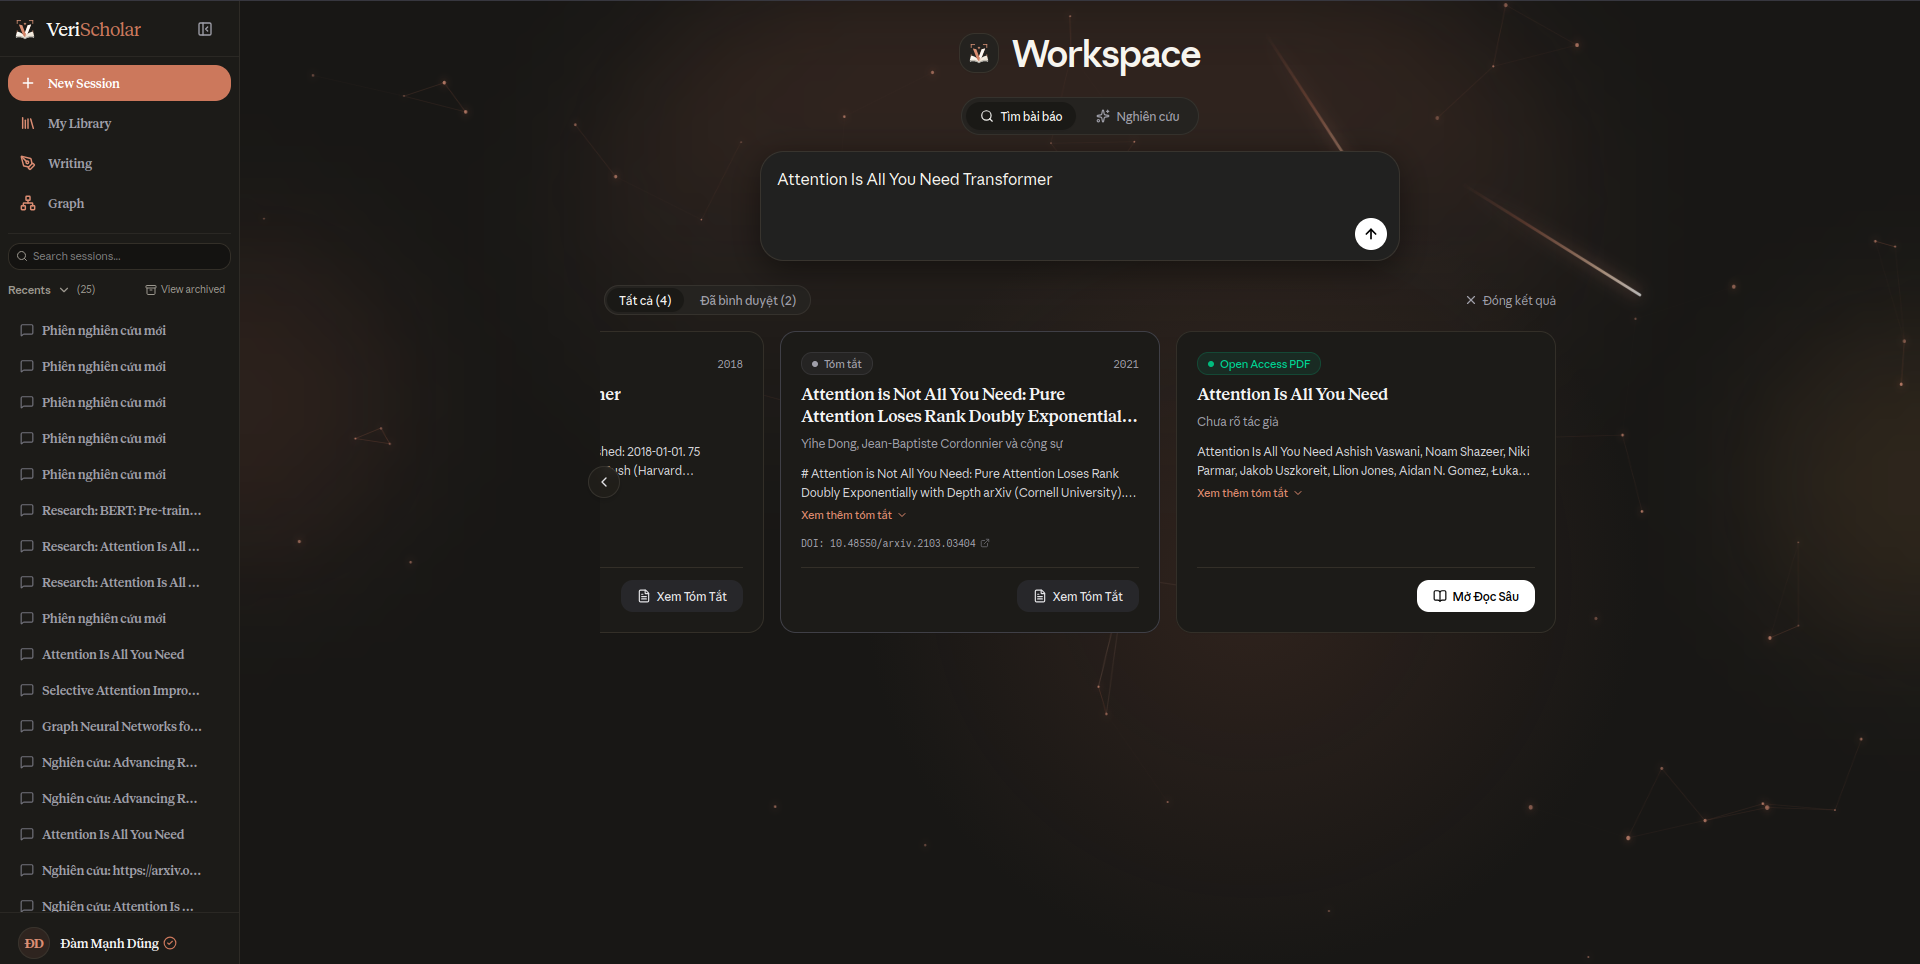
\includegraphics[width=0.95\textwidth]{figures/frontend/search_paper.png}
\caption{Giao diện tìm kiếm và khám phá tài liệu học thuật}
\label{fig:ui_search_paper}
\end{figure}
\FloatBarrier

\subsection{Giao diện quản lý thư viện nghiên cứu cá nhân}
\label{subsubsec:ui_my_library}

Giao diện Thư viện tài liệu nghiên cứu cá nhân cho phép học giả tổ chức, phân loại và lưu trữ hàng nghìn tài liệu khoa học một cách khoa học (Hình~\ref{fig:ui_my_library}):
\begin{itemize}[noitemsep, topsep=2pt]
    \item Cấu trúc thư mục phân cấp theo đề tài: Học giả có thể tạo các thư mục chuyên đề với màu sắc nhận diện trực quan, kéo--thả bài báo giữa các thư mục và quản lý trạng thái phân loại linh hoạt.
    \item Deduplication lưu trữ theo nội dung (CAS): Khi người dùng tải tài liệu PDF qua hộp thoại kéo--thả, hệ thống tính toán mã băm SHA-256 của nội dung tệp. Nếu tệp đã tồn tại trong kho lưu trữ, hệ thống chỉ tạo bản ghi liên kết logic mà không sao chép thêm dữ liệu nhị phân trên đĩa cứng, giúp loại bỏ hoàn toàn các bản sao dư thừa khi nhiều học giả cùng tải lên một ấn phẩm chuẩn (tỷ lệ tiết kiệm thực tế đạt $\frac{K-1}{K}$ với $K$ lượt tải trùng và đạt tới 98\% trong kịch bản lớp học 50 người dùng chung giáo trình).
    \item Quản lý trạng thái xử lý phân đoạn: Bảng danh sách bài báo hiển thị rõ số trang, số lượng phân đoạn đã trích xuất (Chunks), thời điểm tải tệp và tính năng gắn sao đánh dấu các công trình nghiên cứu trọng tâm.
\end{itemize}

\begin{figure}[H]
\centering
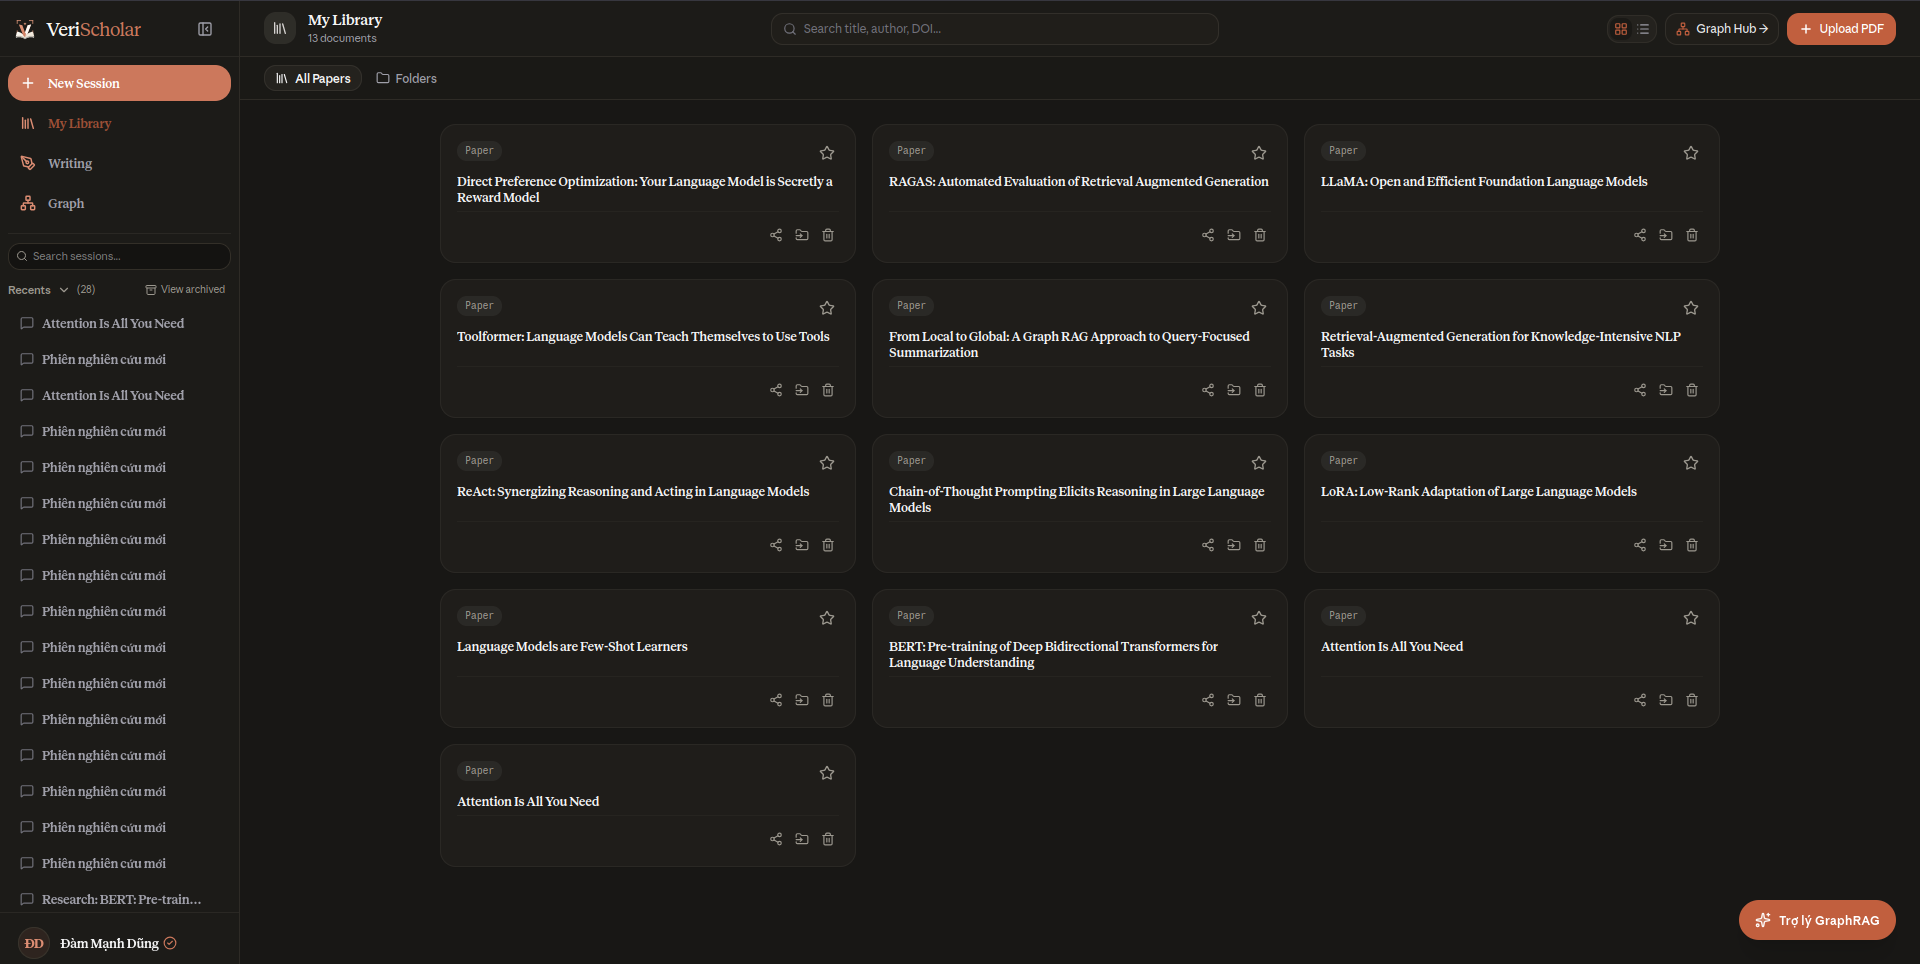
\includegraphics[width=0.95\textwidth]{figures/frontend/my_library.png}
\caption{Giao diện quản lý thư viện nghiên cứu cá nhân}
\label{fig:ui_my_library}
\end{figure}
\FloatBarrier

\subsection{Giao diện đọc sâu tài liệu PDF hai cột và Bounding Box viền vàng}
\label{subsec:ui_deep_reading}

Phân hệ Đọc sâu là không gian làm việc trọng tâm hỗ trợ học giả phân tích, đối thoại và kiểm chứng trực tiếp từng luận điểm của bài báo khoa học (Hình~\ref{fig:ui_deep_read_paper}):
\begin{itemize}[noitemsep, topsep=2pt]
    \item Khung hiển thị kép song song (Dual-pane): Bên trái là trình xem tài liệu PDF Canvas tối ưu hóa cho ấn bản hai cột tiêu chuẩn quốc tế (tự động phân giải và nhận diện bố cục hai cột theo ngưỡng phân cách tọa độ trang); bên phải là khung hội thoại trợ lý AI tương tác theo luồng dữ liệu thời gian thực Server-Sent Events (SSE).
    \item Định vị tự động qua thẻ nguồn trích dẫn và Tô sáng Bounding Box viền vàng: Trong khung hội thoại bên phải (Hình~\ref{fig:ui_deep_read_paper}), mỗi phản hồi suy luận đều đính kèm các thẻ chip nguồn trích dẫn tương tác (ví dụ \texttt{[ $\hookrightarrow$ Attention Is All You Need ]}) cùng chỉ mục minh chứng số ($[1]$, $[2]$) liên kết trực tiếp tới cấu trúc dữ liệu tọa độ của phân đoạn gốc. Khi học giả nhấp chuột vào thẻ nguồn trích dẫn hoặc chỉ mục số, trình xem PDF Canvas bên trái lập tức cuộn mượt đến đúng trang chứa đoạn văn bản minh chứng và kích hoạt lớp phủ đồ họa vẽ khung viền vàng bao quanh đoạn trích gốc trên trang bài báo PDF hai cột.
    \item Độ chính xác hình học cao: Khung Bounding Box đạt chỉ số chồng lấn thực nghiệm trung bình $\text{IoU} \ge 0{,}85$ (kết quả đo lường thực tế đạt $0{,}88$), thời gian định vị dưới 1 giây, giảm thiểu đáng kể công sức đọc dò thủ công trên các ấn phẩm nhiều trang.
\end{itemize}

\begin{figure}[H]
\centering
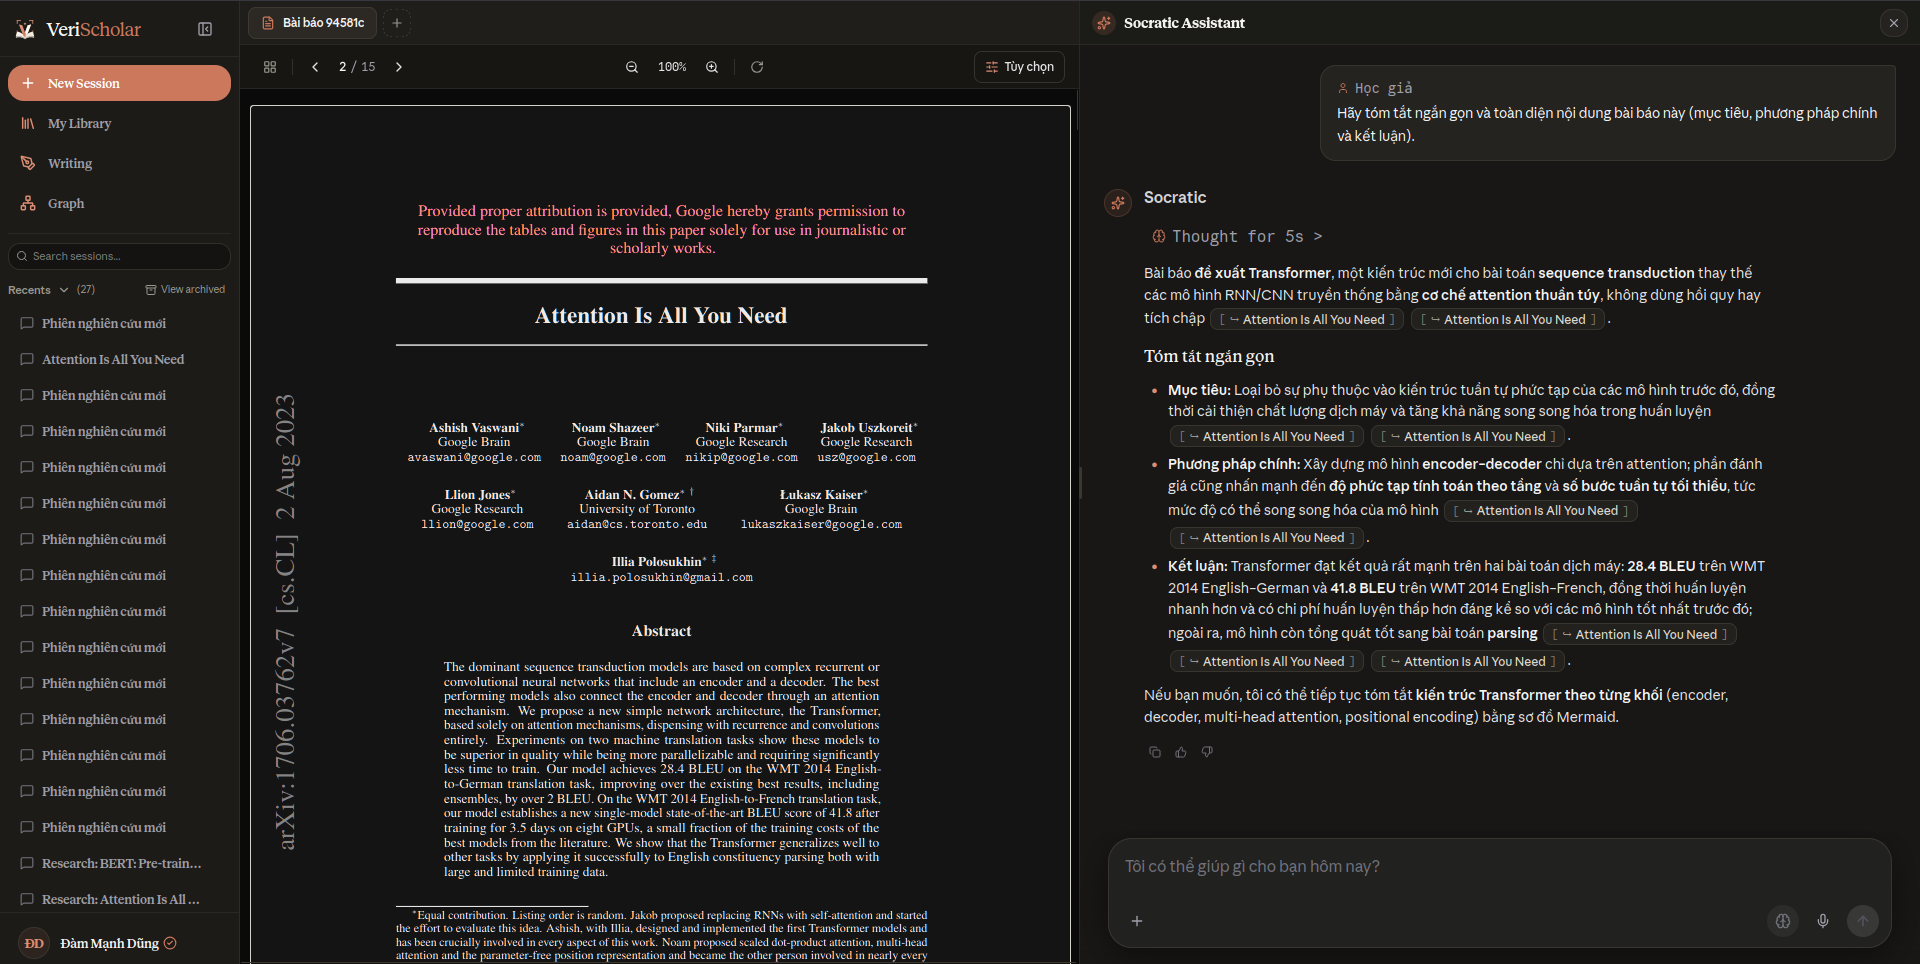
\includegraphics[width=0.95\textwidth]{figures/frontend/deep_read_paper.png}
\caption{Giao diện đọc sâu tài liệu PDF hai cột và Bounding Box viền vàng}
\label{fig:ui_deep_read_paper}
\end{figure}
\FloatBarrier

\subsection{Giao diện mạng đồ thị tri thức 4 thực thể GraphRAG}
\label{subsubsec:ui_graph}

Giao diện mạng đồ thị tri thức học thuật trực quan hóa không gian liên kết ngữ nghĩa giữa các công trình khoa học (Hình~\ref{fig:ui_graph}). Mạng lưới đồ thị thể hiện 4 loại thực thể cốt lõi theo mã màu học thuật chuyên biệt: Bài báo (Paper), Phương pháp (Method), Tập dữ liệu (Dataset), và Kết quả độ đo thực nghiệm (MetricResult). Để hỗ trợ học giả đối chiếu ngay với các công trình nền tảng của lĩnh vực trí tuệ nhân tạo khi khởi tạo không gian làm việc, hệ thống nạp sẵn tập dữ liệu hạt giống gồm 12 bài báo kinh điển (12 Landmark Papers Seed Corpus, bao gồm 58 đỉnh thực thể, 111 cạnh quan hệ và 15 trang tóm tắt tổng quan Graph Wiki biên dịch sẵn) kết hợp cùng các tài liệu PDF do người dùng tải lên trong thư viện cá nhân. Học giả có thể tương tác trực quan bằng cách phóng to, thu nhỏ, kéo thả các đỉnh để khám phá các cụm chuyên đề phân hoạch bằng thuật toán Louvain, nhận diện khoảng trống nghiên cứu (Research Gaps) và thực hiện các truy vấn so sánh liên tài liệu tức thời. Bên cạnh đó, đồ thị hỗ trợ cơ chế lọc tương tác và tìm kiếm thực thể nhanh chóng, giúp định vị các công trình cốt lõi một cách thuận tiện.

\begin{figure}[H]
\centering
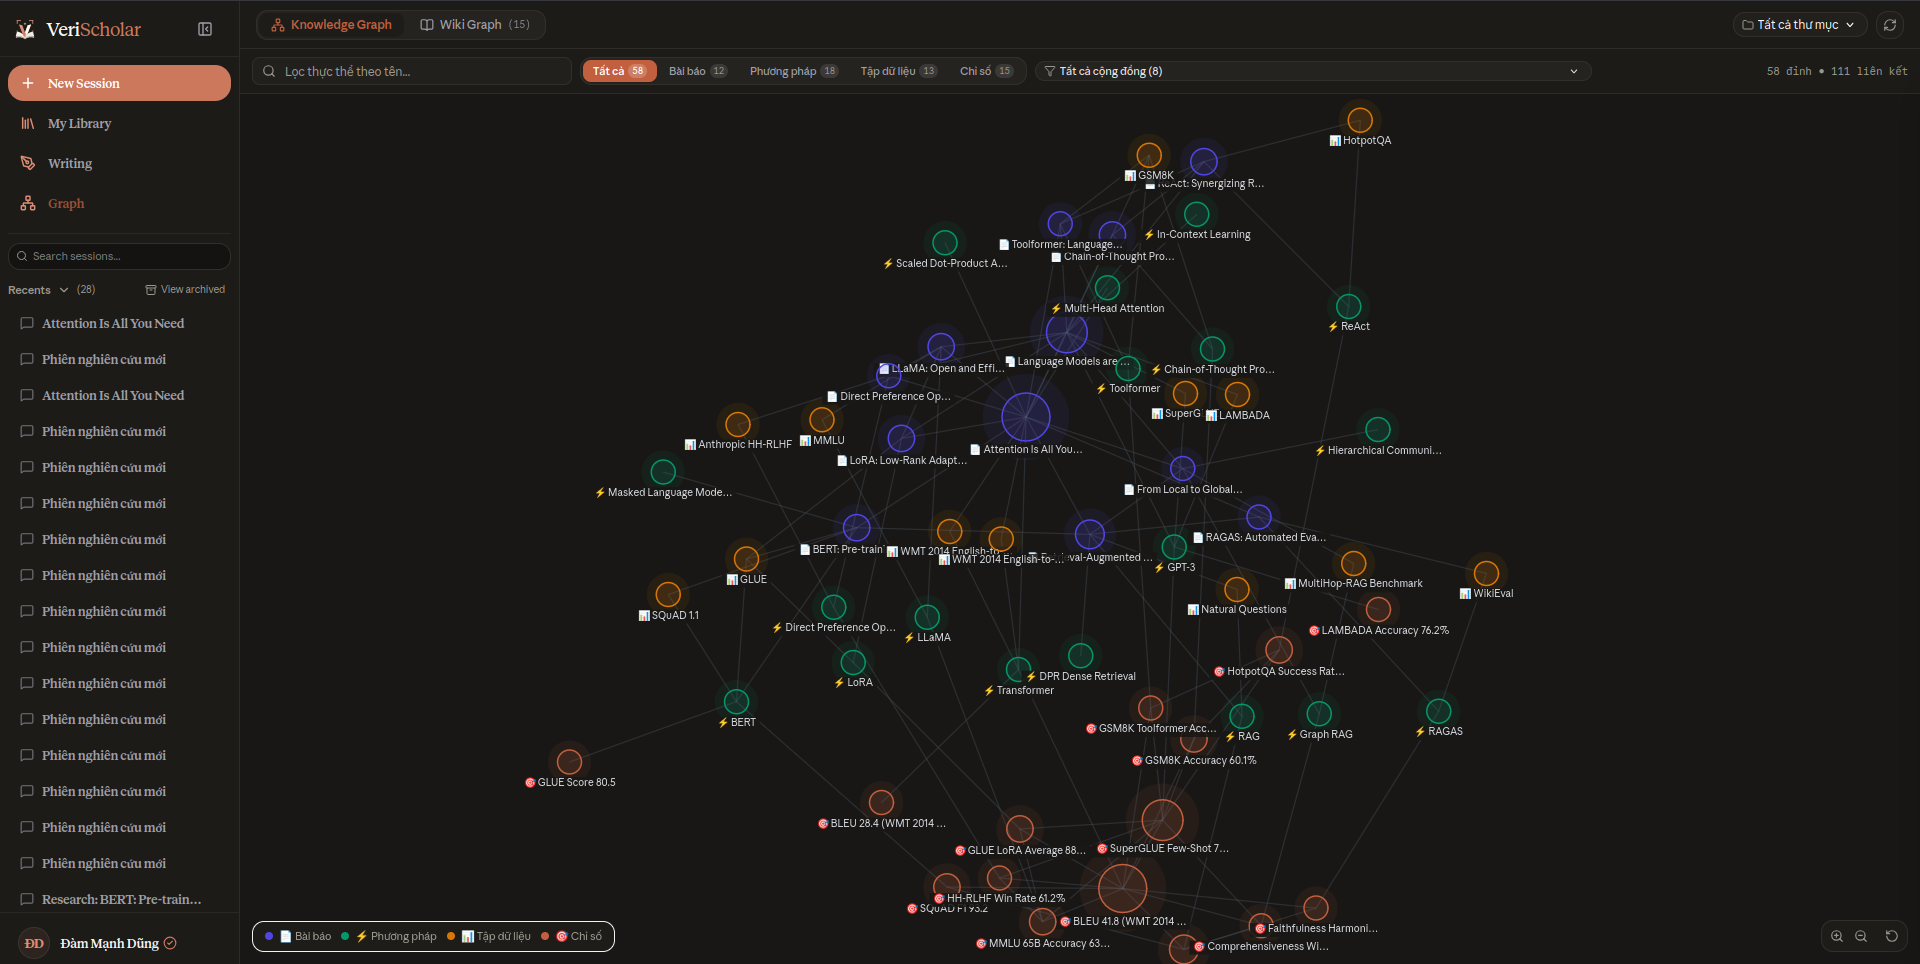
\includegraphics[width=0.95\textwidth]{figures/frontend/graph.png}
\caption{Giao diện mạng đồ thị tri thức học thuật 4 thực thể GraphRAG}
\label{fig:ui_graph}
\end{figure}
\FloatBarrier

\subsection{Giao diện kho khóa API cá nhân (BYOK) và hồ sơ học giả}
\label{subsec:ui_profile}

Giao diện Quản lý hồ sơ học giả và Kho khóa API cá nhân bảo đảm quyền tự chủ dữ liệu và tính an toàn thông tin tuyệt đối cho nhà nghiên cứu (Hình~\ref{fig:ui_byok}):
\begin{itemize}[noitemsep, topsep=2pt]
    \item Định danh học giả quốc tế ORCID iD: Hỗ trợ liên kết tài khoản với mã định danh quốc tế chuẩn ISO 27729 (ORCID iD gồm 16 chữ số). Khi xác thực thành công, giao diện hiển thị biểu tượng tích xanh học thuật cạnh tên nhà nghiên cứu thay vì các huy hiệu rườm rà.
    \item Kho khóa API bảo mật cá nhân (BYOK): Cho phép học giả cấu hình khóa API riêng (OpenAI, Anthropic, Google Gemini) theo cơ chế ``Mang khóa bí mật của chính bạn''. Khóa API được gửi qua kết nối TLS tới máy chủ, mã hóa xác thực ở trạng thái lưu trữ (at-rest) bằng thuật toán đối xứng AES-256-GCM (chỉ lưu bản mã kèm vector khởi tạo IV vào cột \texttt{encrypted\_key} của bảng \texttt{user\_api\_keys}, trong khi khóa chủ KEK được cô lập trong biến môi trường máy chủ/KMS). Khi phát sinh yêu cầu suy luận, khóa chỉ được giải mã tạm thời trên bộ nhớ khả biến (RAM) trong phạm vi hàm thực thi và giải phóng ngay sau khi đóng luồng SSE, cam kết không bao giờ lưu khóa ở dạng văn bản thuần (plaintext) xuống đĩa cứng hay nhật ký hệ thống.
\end{itemize}

\begin{figure}[H]
\centering
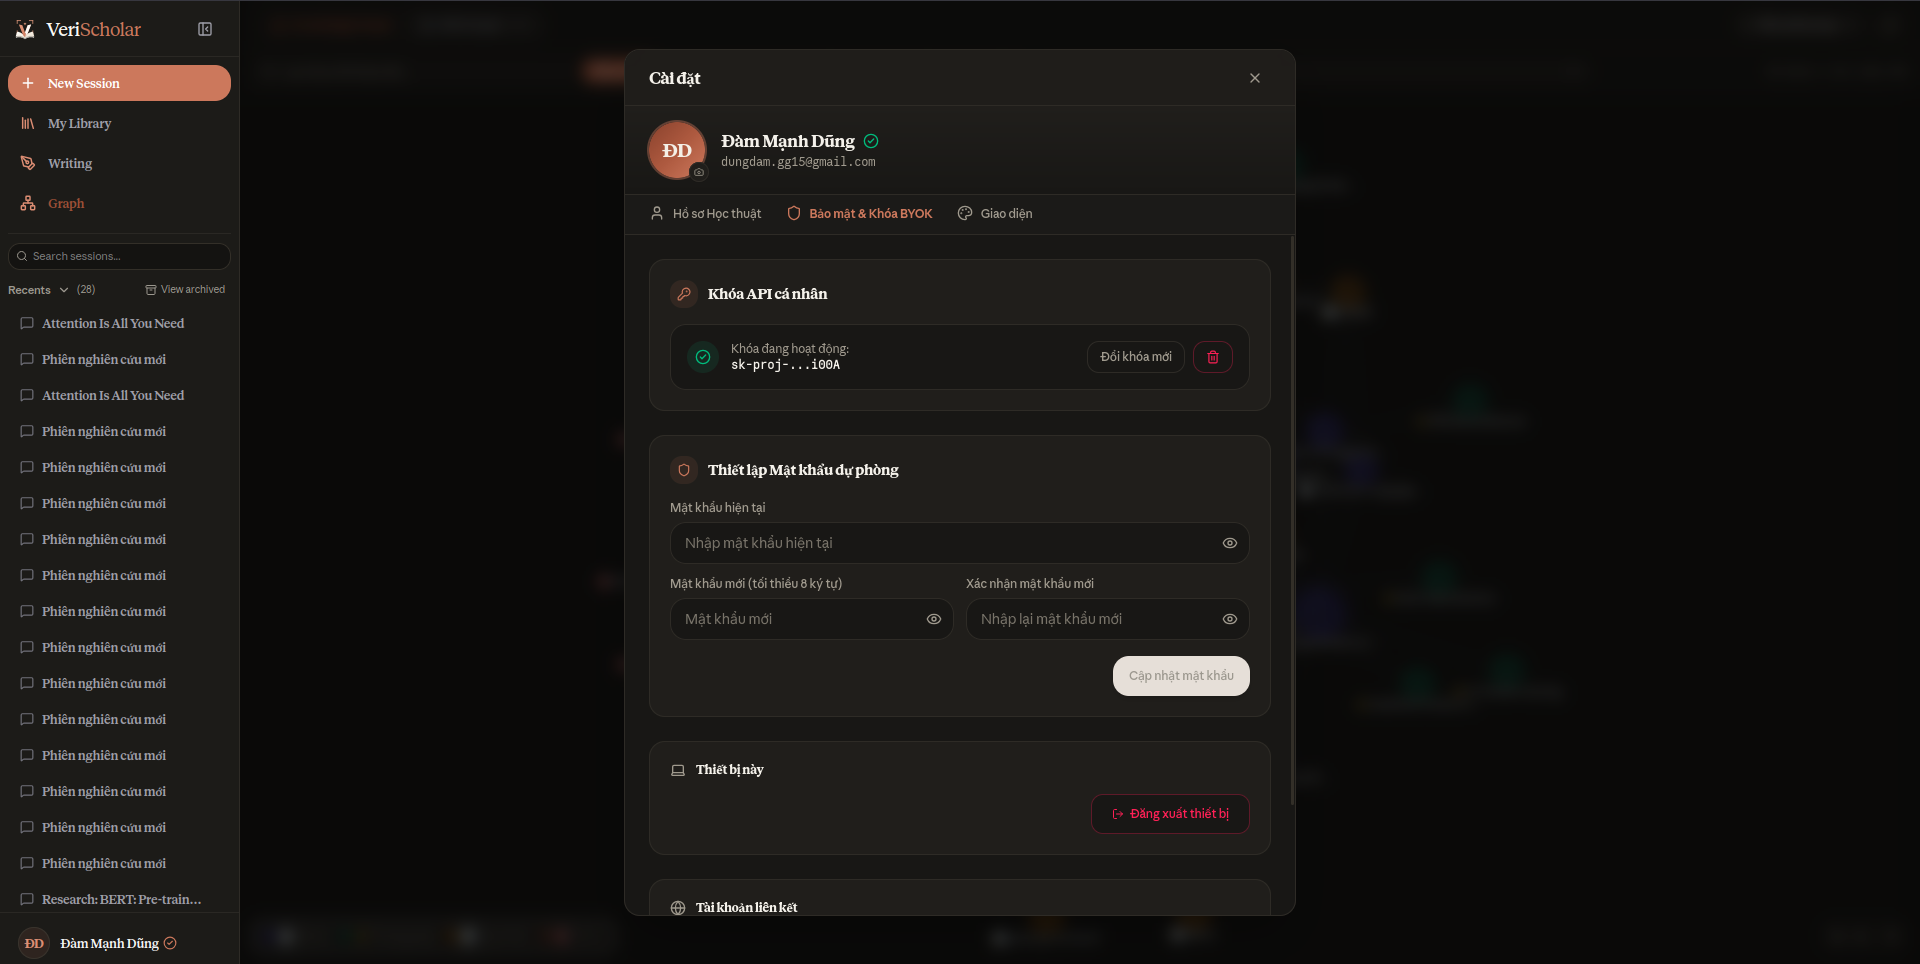
\includegraphics[width=0.75\textwidth]{figures/frontend/byok.png}
\caption{Giao diện kho khóa API cá nhân (BYOK) và hồ sơ học giả}
\label{fig:ui_byok}
\end{figure}
\FloatBarrier

\subsection{Giao diện soạn thảo bản thảo bài báo LaTeX và tự sửa lỗi biên dịch}
\label{subsec:ui_writing}

Phân hệ Soạn thảo và Tự sửa lỗi là bước hoàn thiện cuối cùng trong chu trình nghiên cứu khoa học của VeriScholar (Hình~\ref{fig:ui_writing_paper}):
\begin{itemize}[noitemsep, topsep=2pt]
    \item Môi trường soạn thảo chuyên dụng với Monaco Editor: Giao diện tích hợp trình biên tập mã nguồn Monaco Editor, cung cấp đầy đủ tiện ích tô màu cú pháp LaTeX, gợi ý lệnh tự động, quản lý cây thư mục dự án đa tệp (\texttt{main.tex}, \texttt{references.bib}, thư mục ảnh) và khung xem trước tài liệu PDF thời gian thực.
    \item Biên dịch cô lập trong môi trường E2B MicroVM: Toàn bộ tiến trình biên dịch TeX Live được chuyển giao thực thi cách ly hoàn toàn bên trong E2B Sandbox MicroVM, khởi tạo chỉ trong 150 mili-giây, ngăn chặn hoàn toàn nguy cơ tấn công an ninh mạng qua mã macro LaTeX.
    \item Chu trình tự sửa lỗi ReAct (Autonomous Healing Loop): Khi quá trình biên dịch phát sinh lỗi cú pháp, AI Agent tự động kích hoạt chu trình ReAct: đọc nhật ký lỗi $\to$ lập luận suy diễn nguyên nhân $\to$ tạo bản vá vi phẫu (Surgical Diff) sửa lỗi mã nguồn, đạt tỷ lệ tự sửa lỗi biên dịch thành công vượt trên 90\%.
\end{itemize}

\begin{figure}[H]
\centering
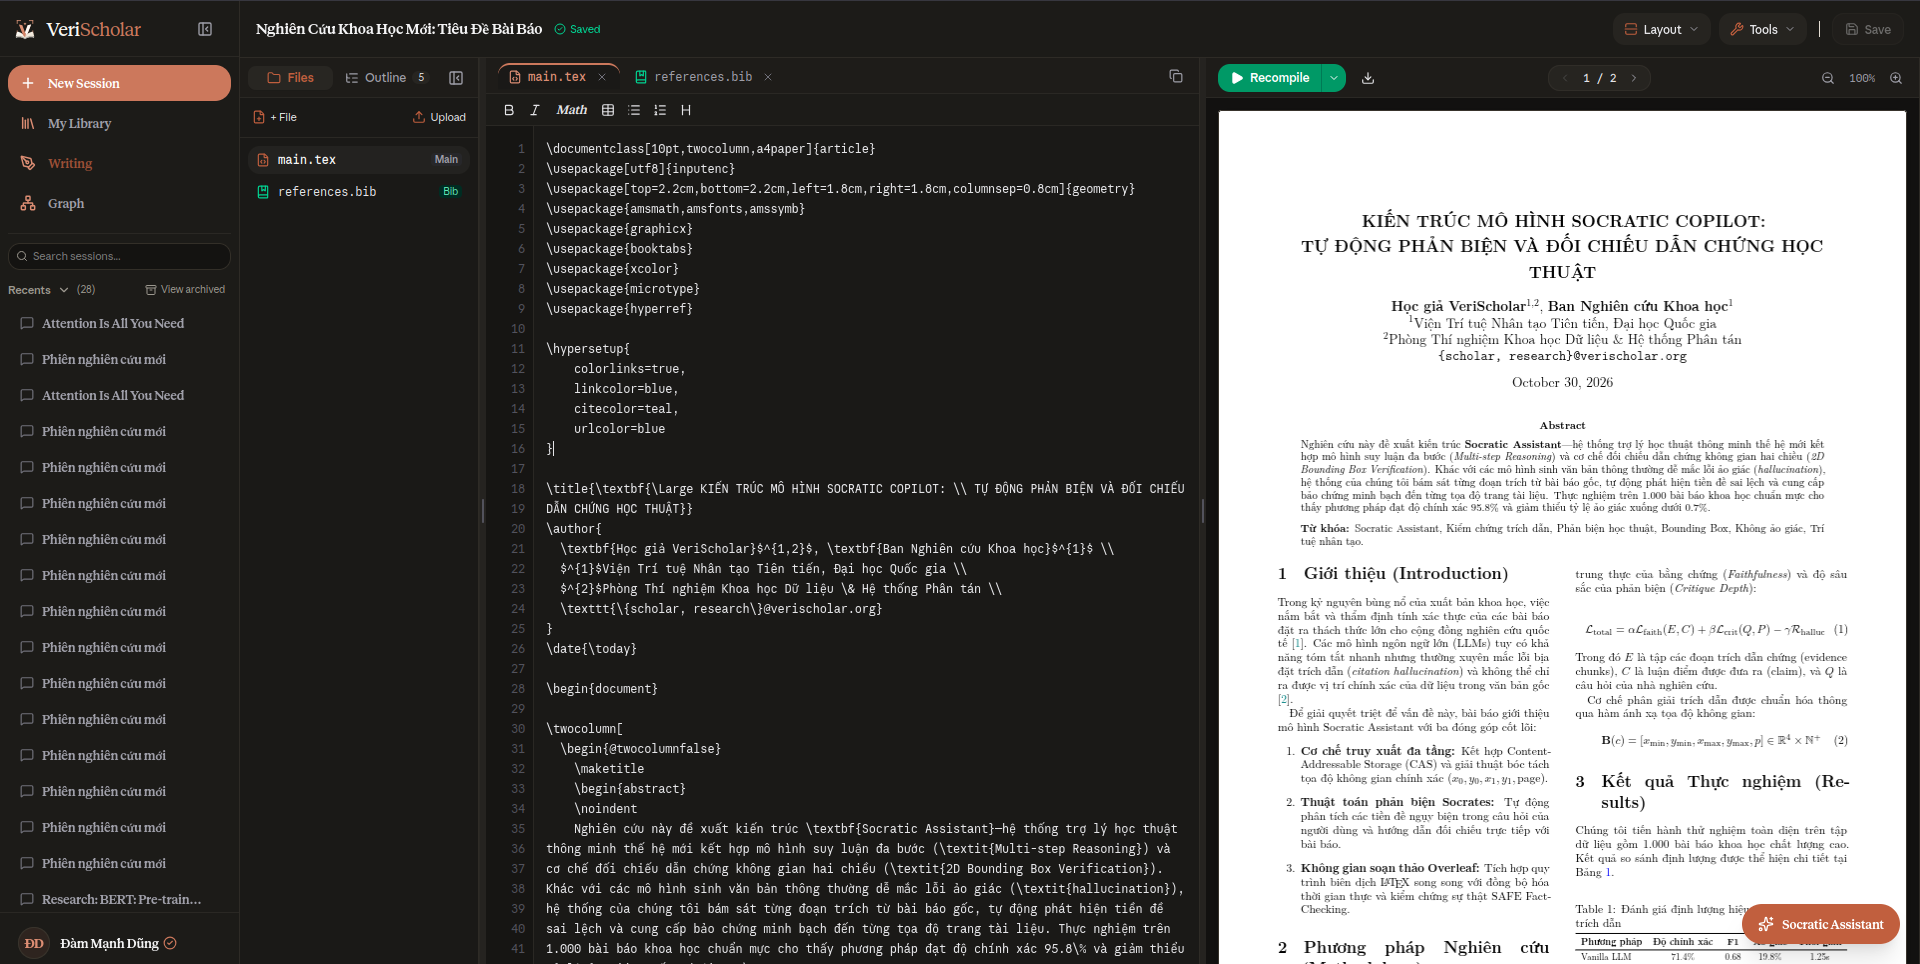
\includegraphics[width=0.95\textwidth]{figures/frontend/writing_paper.png}
\caption{Giao diện soạn thảo bản thảo bài báo LaTeX và tự sửa lỗi biên dịch}
\label{fig:ui_writing_paper}
\end{figure}
\FloatBarrier

